%author: yjw, 2024-4-1
%\subsection{关键设计}
本项目核心目标是将自动模糊测试(Fuzzing)框架迁移到ROS2系统上,并且针对ROS2特性对测试效率做出改进提升。
具体而言,我们试图寻找更多可能的程序输入口,使测试覆盖的输入可能性尽可能多;尝试构造质量尽可能高的初始种子;
寻找更多反馈信息,用于监控被测程序(即ROS2节点)的内部状态,以更高效地指导对输入的变异;
尝试模拟更多ROS2执行环境,模拟程序可能遇到的各种实际情况。

\subsubsection{多维度输入}
\subsubsection{程序插桩}
\subsubsection{测试加速}


最终,给出本项目的核心框架如图\ref{pic:off}。

\begin{figure}[h]
    \centering
    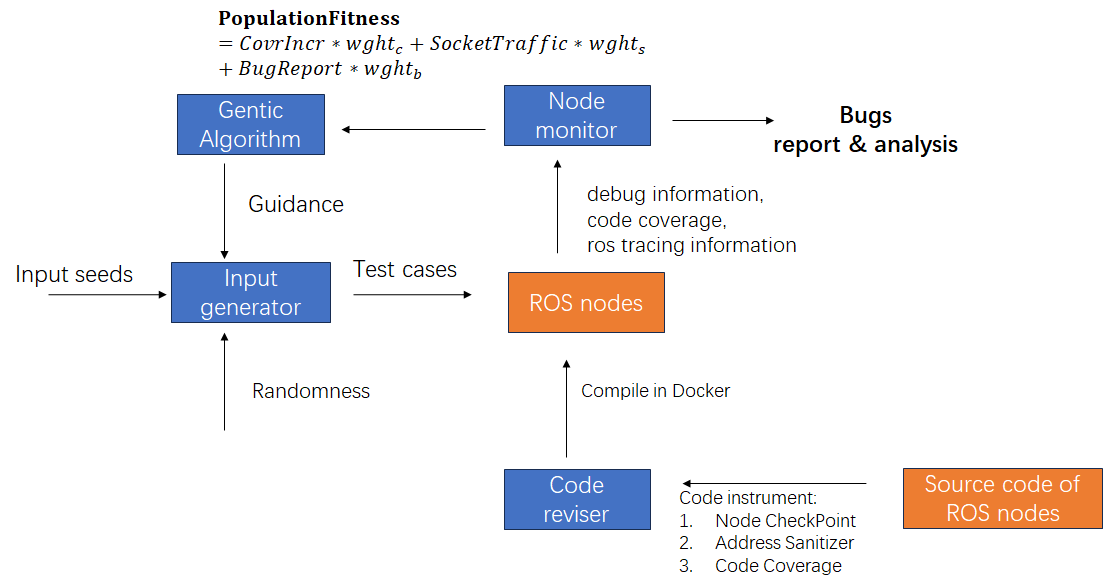
\includegraphics[width=14cm]{our_fuzz_framework.png}
    \caption{本项目实现的Fuzz框架}
    \label{pic:off}
\end{figure}

\subsubsection{测试环境}